\section{The spin chain}

\subsection{Ground states}\label{sec:groundstates}

In this section we initialise $10$ spins in random directions and simulate the time evolution for $J <0$ and $J>0$. The plots of the $z$-component of each of the spins over time is shown in figure \ref{fig:gs}. What is evident from these plots is that a positive coupling constant $J$ tends to make the spins align with their neighbours, while the negative constant tends to make them oppose them. This is a fact that is readily seen from inspecting the hamiltonian in \eqref{eq:hamiltionian}, since a positive $J$ makes the maximum of $\sum_{j,k} \mathbf{S}_j \cdot \mathbf{S}_k$ most energetically favourable, while a negative one makes its minimum most favourable. These two cases correspond to a ferromagnetic and anti-ferromagnetic system respectively.

The reason for this being apparent when only plotting the $S_z$-component is the non-zero anisotropy-constant $d_z$. As seen from the hamiltonian, setting this positive will favour spins in the $z$-direction. This is also the reason that approximately half of the spins in the case of $J<0$ being directed along $\mathbf{e}_z$ while the others are directed along $-\mathbf{e}_z$.

\begin{figure}[htb]
	\centering
	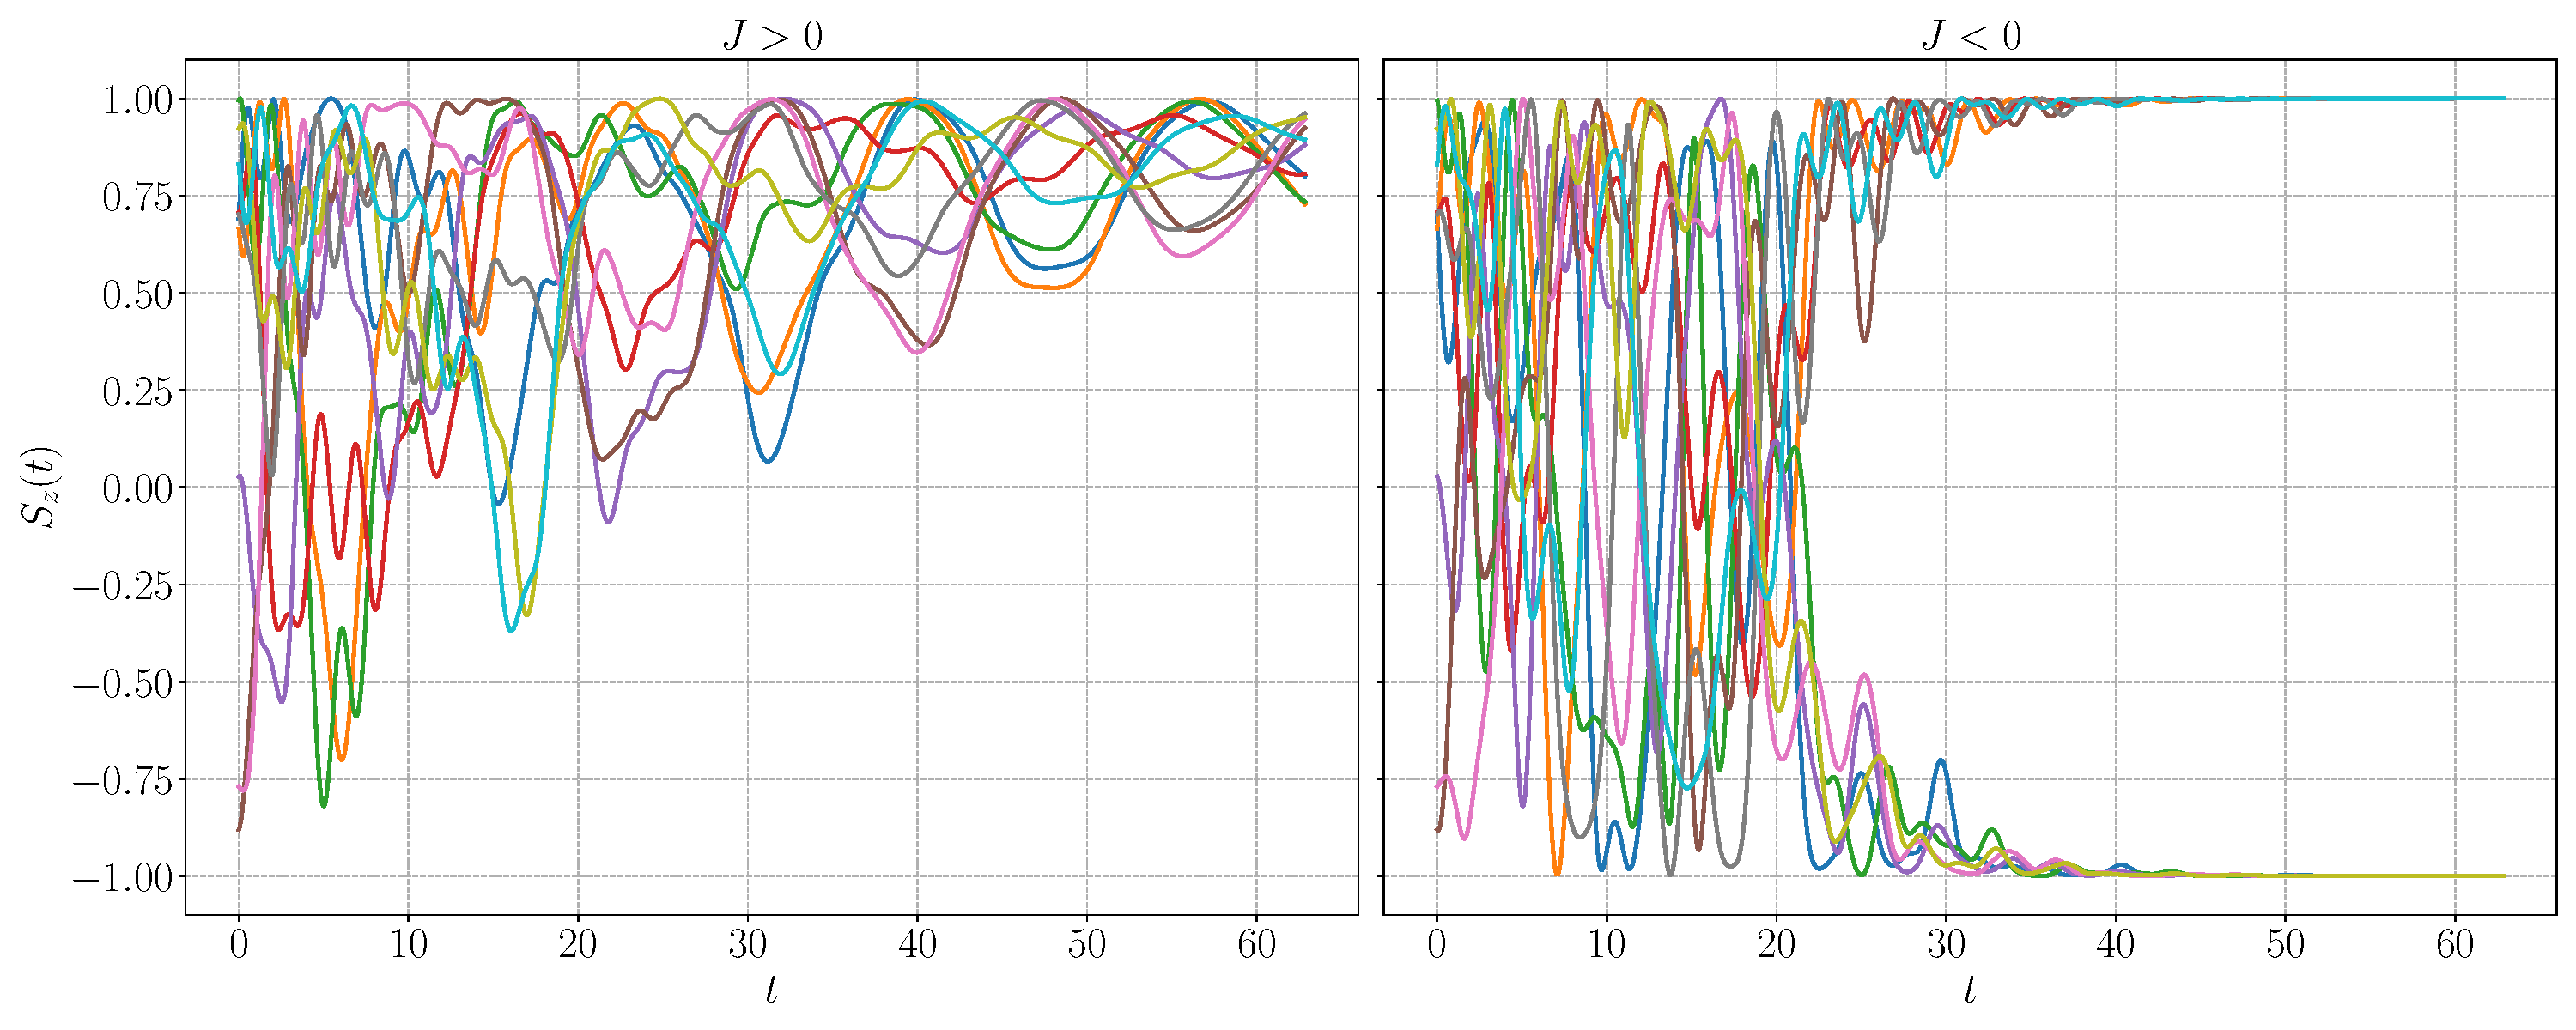
\includegraphics[width=\columnwidth]{../fig/gs.pdf}
	\caption{The figure shows the plot of the $z$-component of $10$ spins in a system of positive and negative coupling constant.}
	\label{fig:gs}
\end{figure}

\subsection{The magnon}

\subsubsection{Uncoupled system}

We initialise the system of $10$ spins with random orientations in space and set $J = 0$, $d_z = 1$, $\alpha = 0$ to demonstrate that all the spins precess in time. The trajectories of the $x$ and $y$ components of the spins is plotted in figure \ref{fig:precessionsxy}

\begin{figure}[htb]
	\centering
	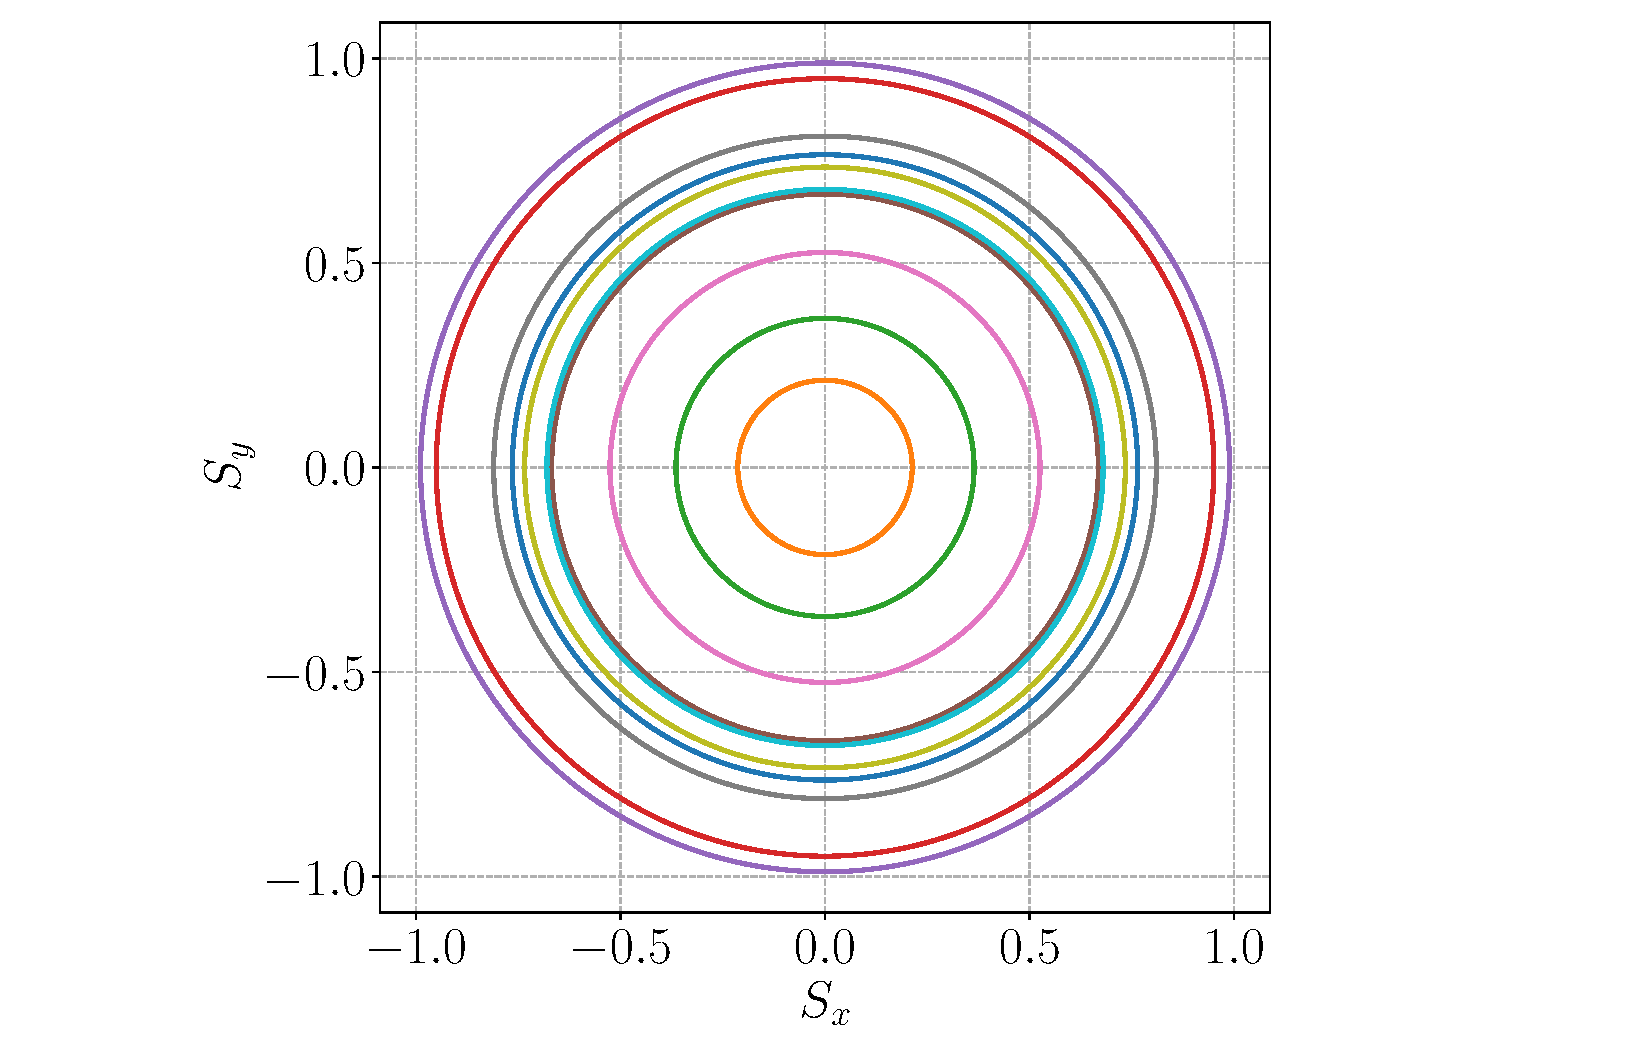
\includegraphics[width=0.8\columnwidth]{../fig/precession_xy.pdf}
	\caption{Trajectories of the $x$ and $y$ components of the $10$ randomly initialised spins.}
	\label{fig:precessionsxy}
\end{figure}

Next, we initialise all the spins along the $z$ direction except for one of them which we tilt slightly. Since there is no coupling between the spins, the precession of the first spin will not affect the others. Furthermore, when $\mathbf{S} = S\mathbf{e}_z$, the right hand side of the LLG \eqref{eq:llg} will be zero since the effective field is $\parallel \mathbf{e}_z$. As expected, this is also what is observed when simulating the system. This is shown in figure \ref{fig:precessions}.

\begin{figure}[htb]
	\centering
	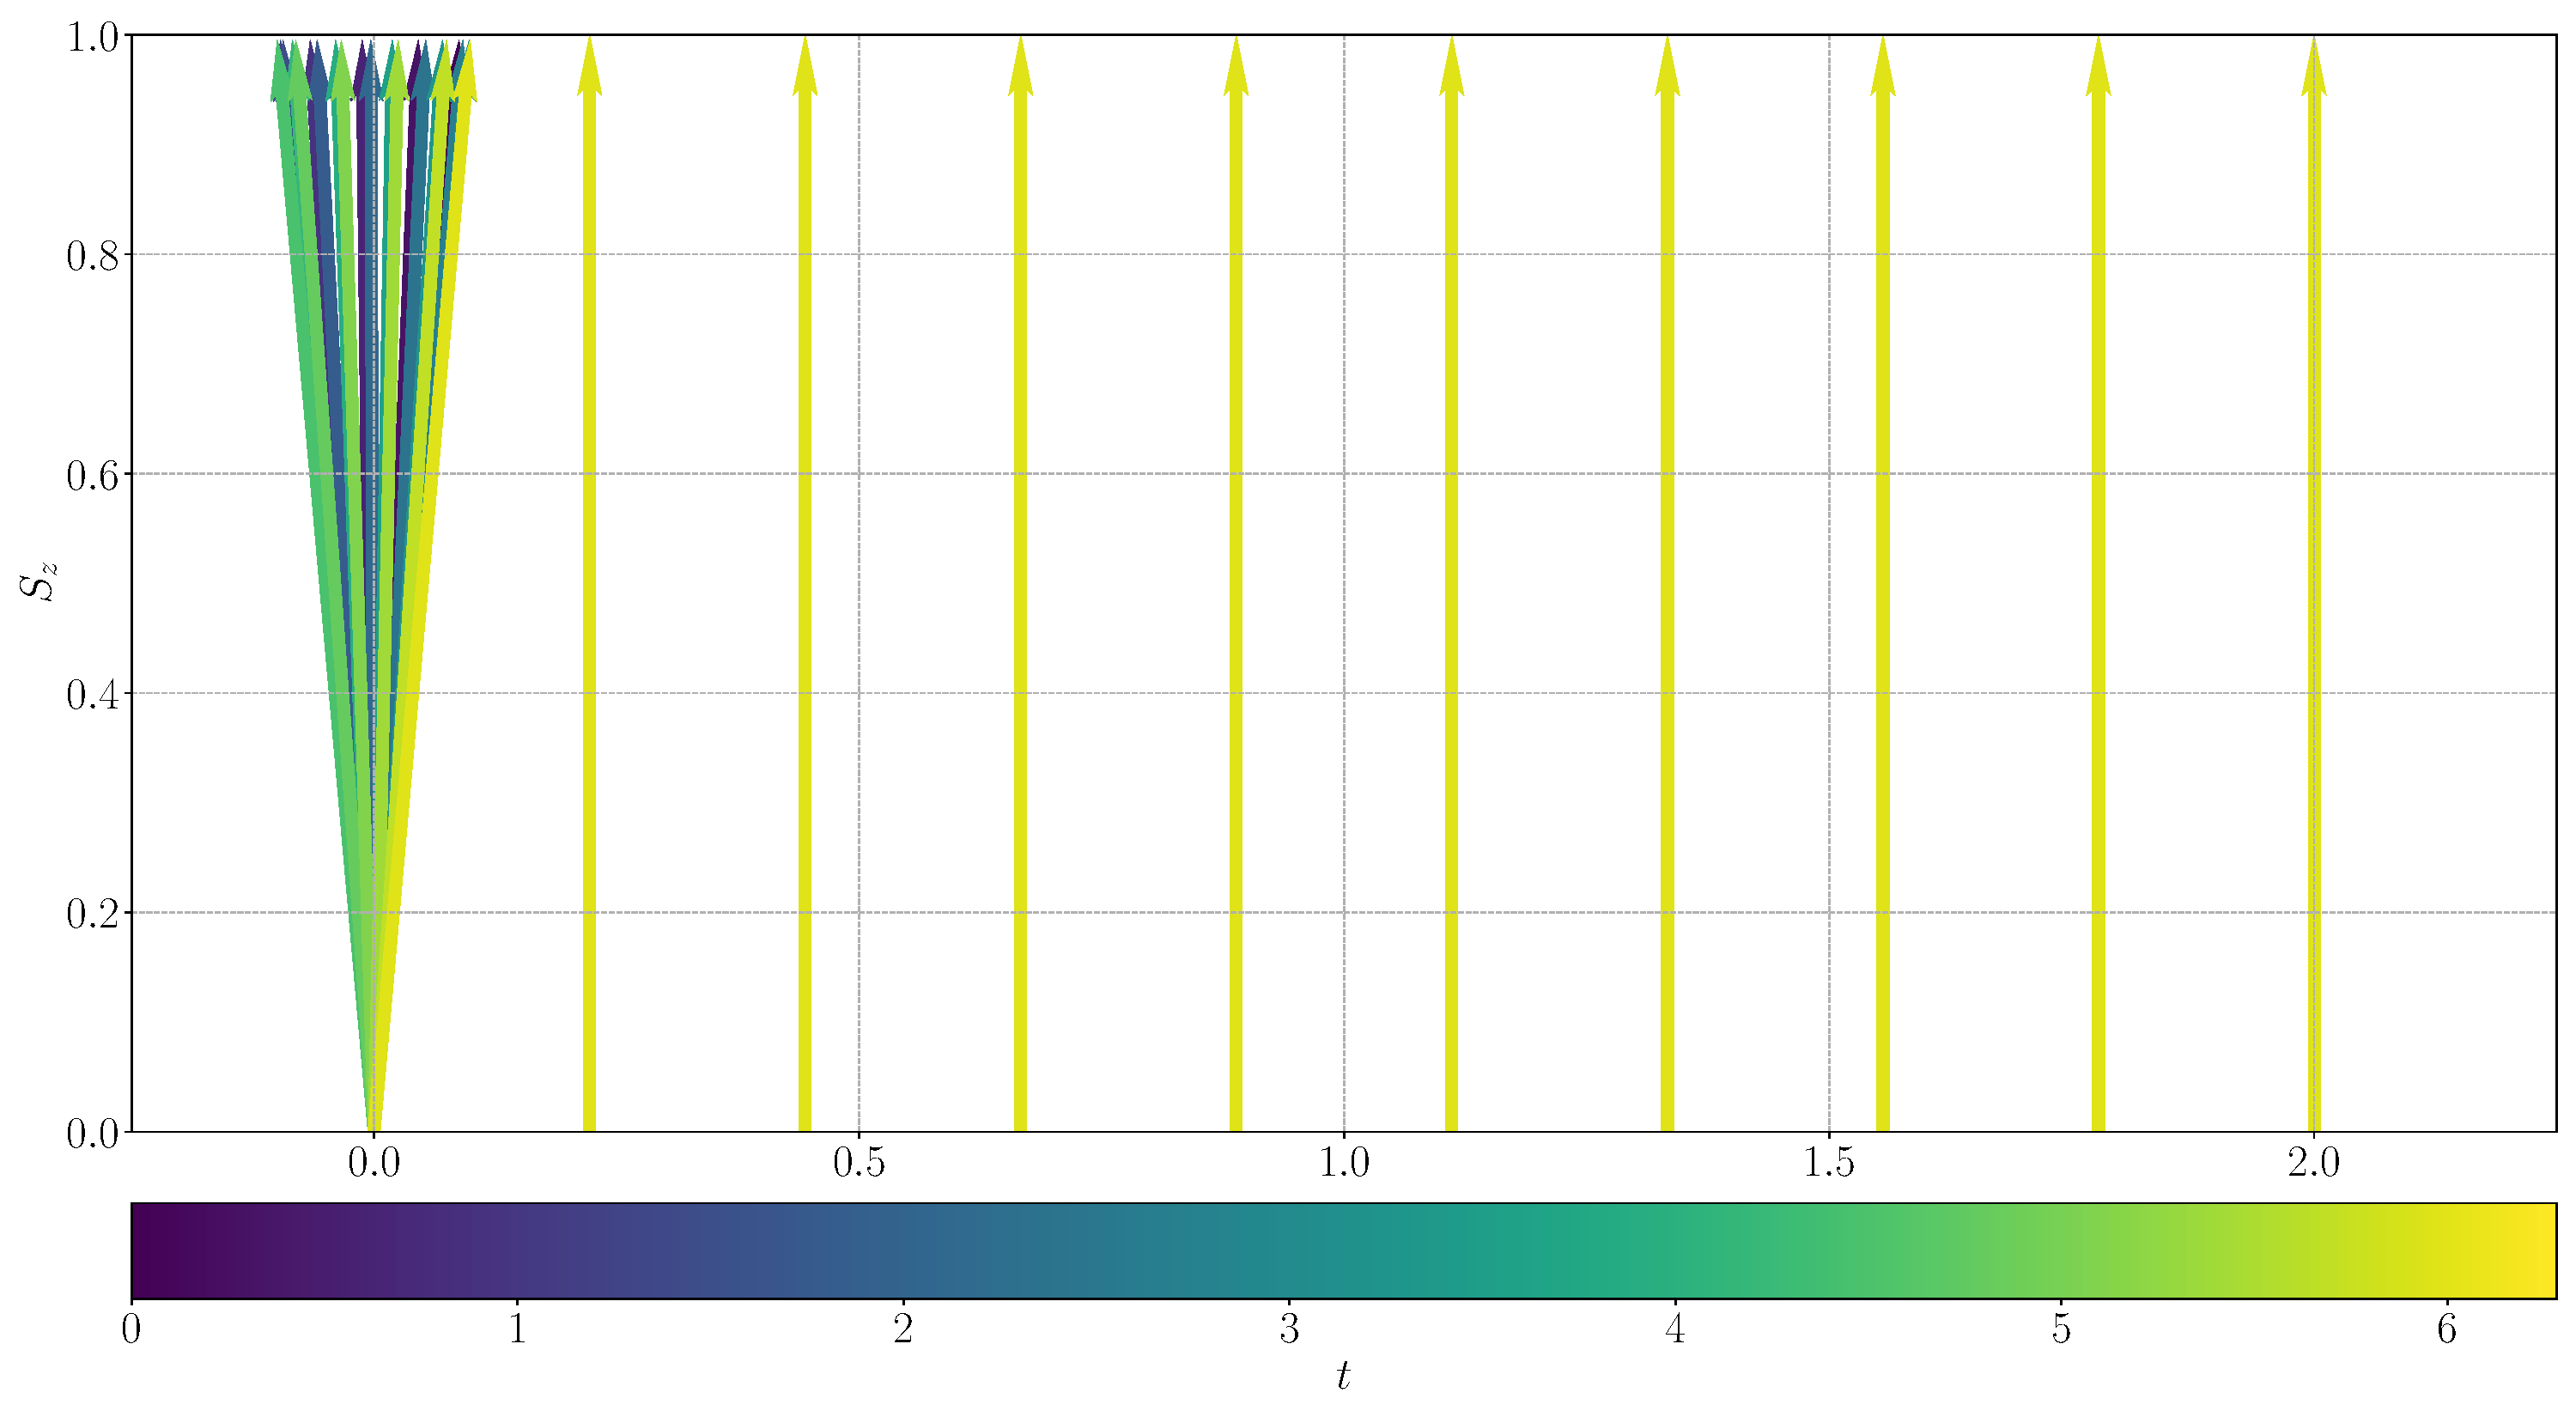
\includegraphics[width=\columnwidth]{../fig/10_precessions.pdf}
	\caption{The figure shows uncoupled oscillations of the spin chain.}
	\label{fig:precessions}
\end{figure}

\subsubsection{Coupled system, $J > 0$}

If we repeat the procedure used in the previous section except that we couple the spins with $J > 0$, we will observe that all the spins will start to precess, even if they are initialised along the $z$-axis. Since the time evolution is hard to catch on a $2\mathrm{d}$ plot I have made a video showing it \href{https://folk.ntnu.no/sondrdl/spinwaves/coupled_spins.mp4}{here}. It is also shown in figure \ref{fig:damped_heat} as a heat map. What is apparent here is that the neighbouring spins couple to each other. Since we are dealing with a finite system, I have chosen to use periodic boundary conditions, so that the first spin affects the last one and vice versa. Implementing this in python requires no effort at all as we can access the left hand neighbour of spin \texttt{i} with \texttt{i-1} regardless of the value of \texttt{i}, and the right hand neighbour with \texttt{(i-1)\%n} where \texttt{n} is the number of spins. This looks a bit artificial in the video, but it corresponds physically to arranging the linear chain in a circle. Another choice of boundary conditions is to simply say that the first and last spin only has \textit{one} neighbour. 

%\begin{figure}[htb]
%	\centering
%	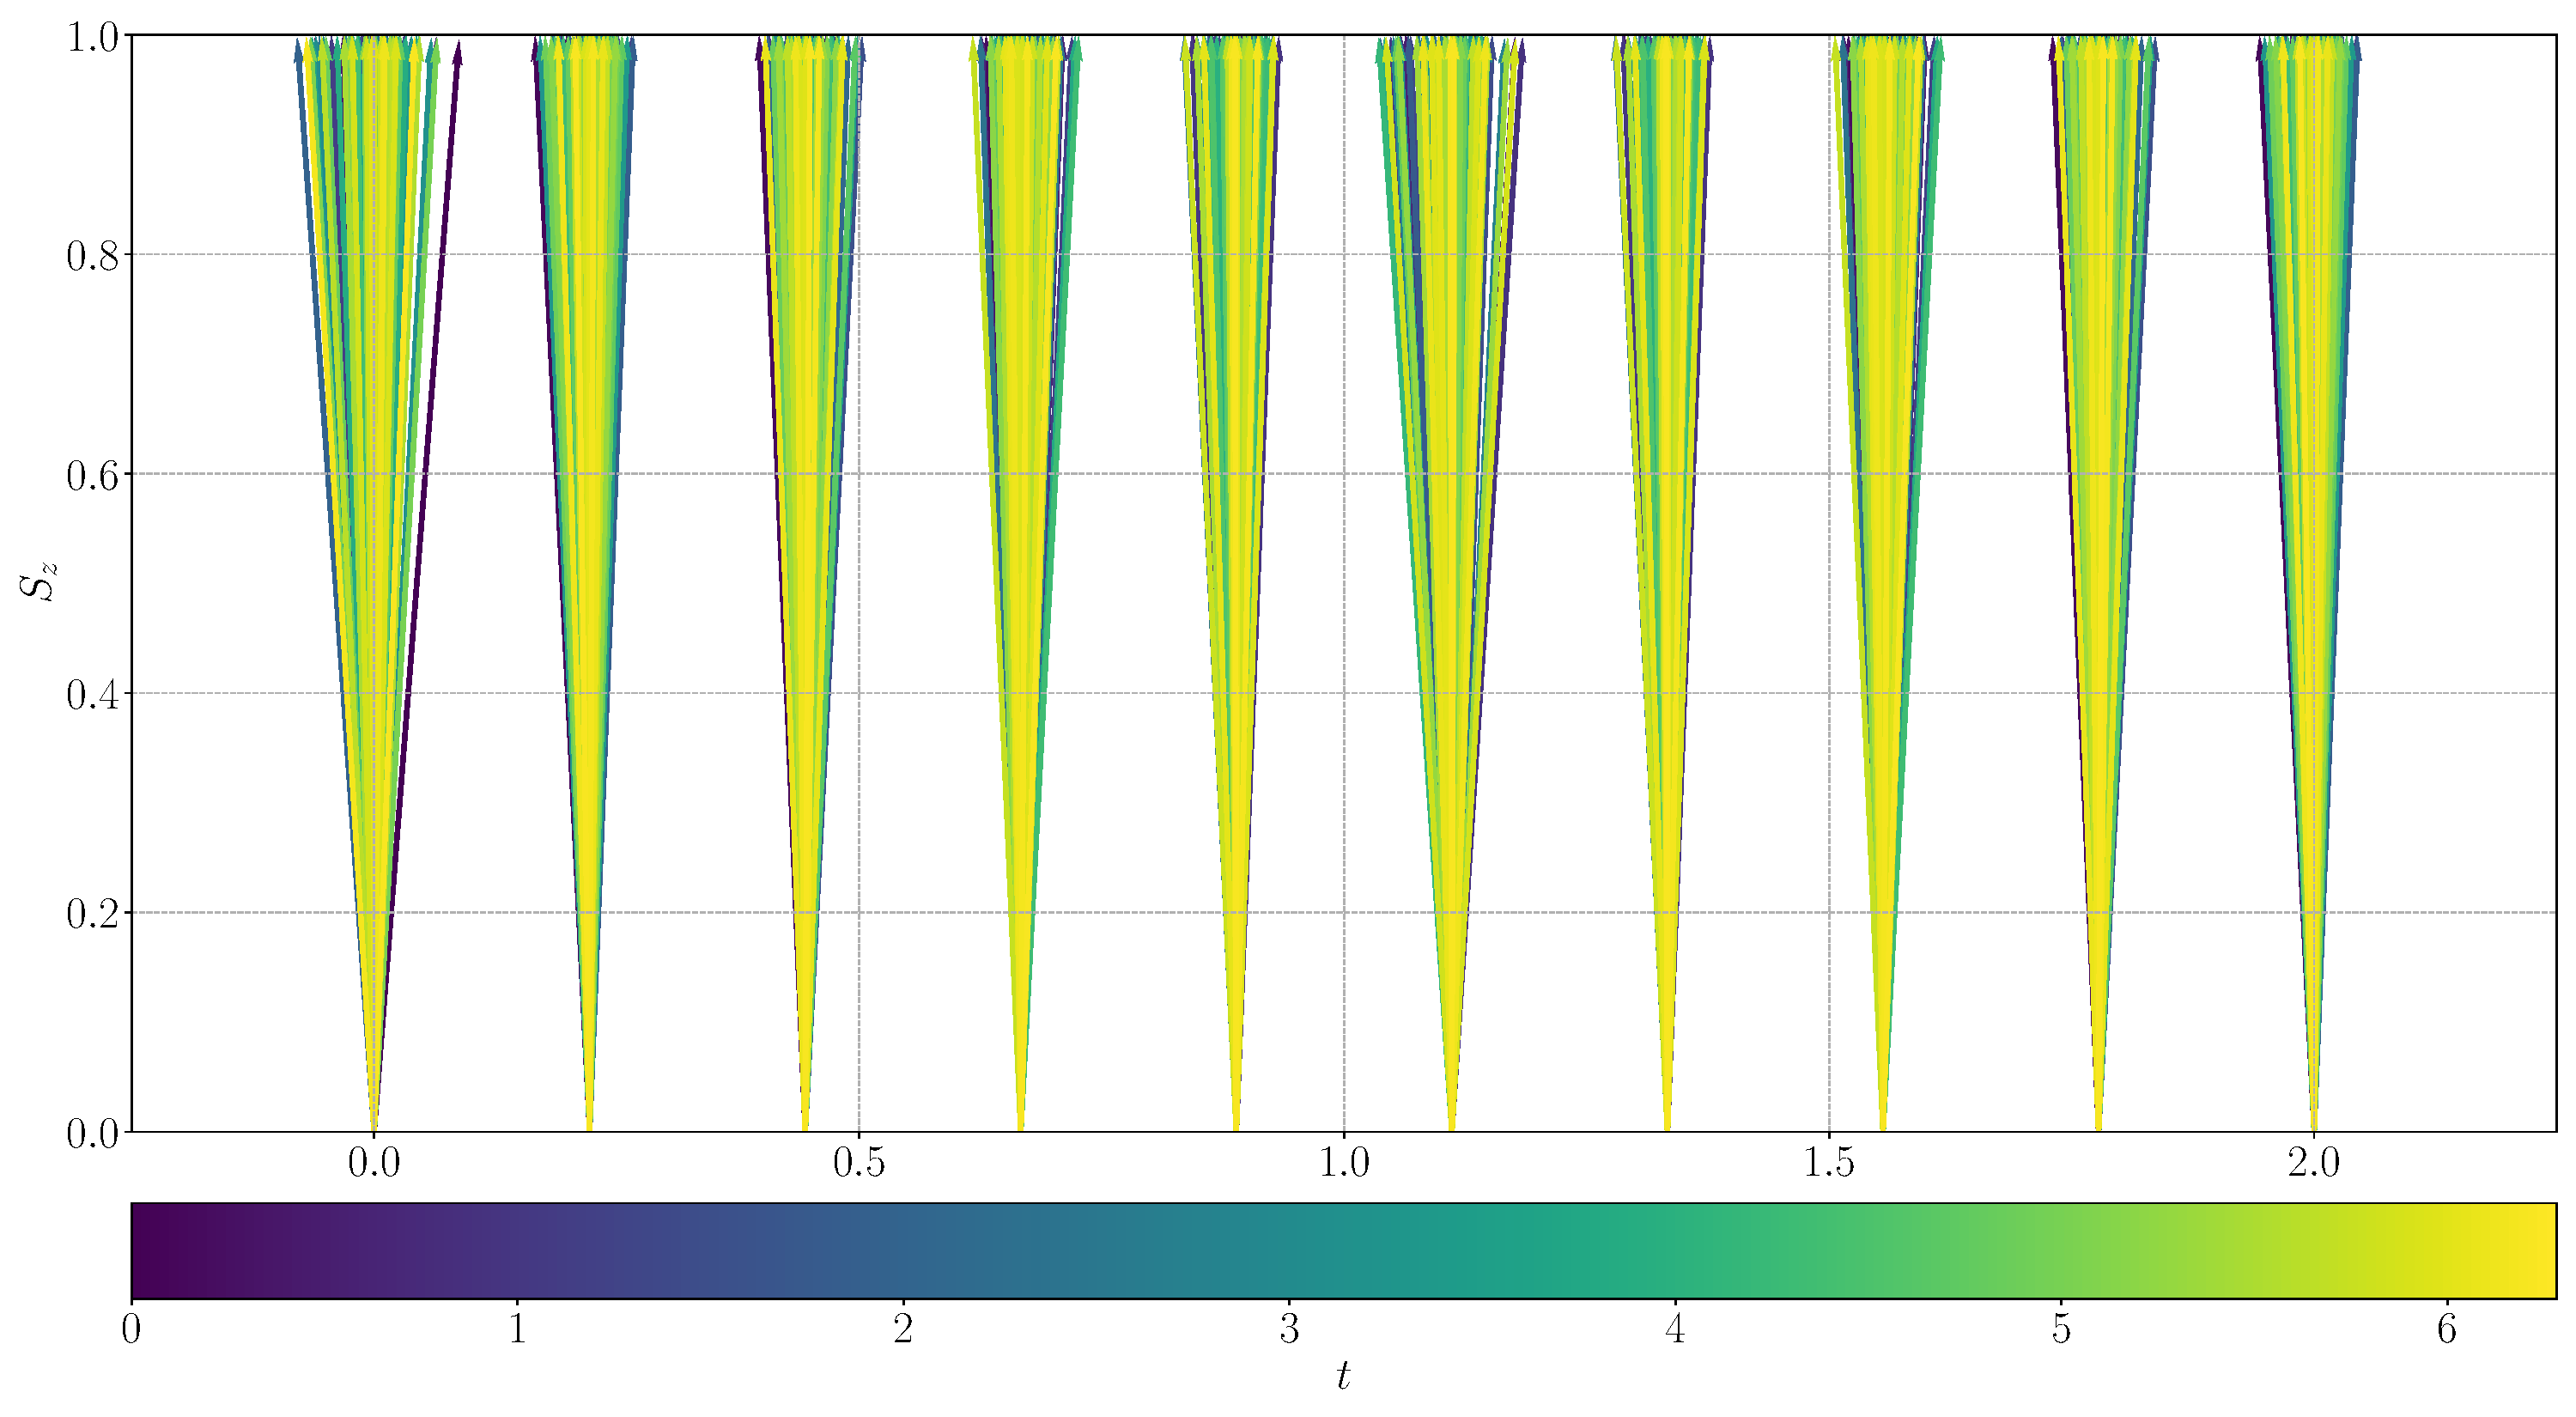
\includegraphics[width=\columnwidth]{../fig/10_precessions_coupled.pdf}
%	\caption{The figure shows coupled oscillations of the spins. A video displaying the same data set can be found \href{https://folk.ntnu.no/sondrdl/spinwaves/coupled_spins.mp4}{here}.}
%	\label{fig:coupled_precessions}
%\end{figure}

If we are to simulate an infinite system we obviously cannot use a discrete model. However, the simulations above suggests that in the limit of \textit{many} spins we can describe the chain as a continuous wave. Then we would have to associate to every index $j$ a position in space 
$$
	\mathbf{S}_j(t) \to \mathbf{S}(\mathbf{x},t) \quad ; \quad j \to \mathbf{x},
$$
where $\mathbf{x}$ is the position of spin $j$.
If we approximate the directional derivatives along a lattice vector $\mathbf{a}$ by the finite differences 
$$
	 \|\mathbf{a}\|^2  \nabla^2 \mathbf{S}(\mathbf{x},t) \approx \|\mathbf{a}\|^2 \frac{\mathbf{S}(\mathbf{x} - \mathbf{a},t) - 2 \mathbf{S}(\mathbf{x},t) + \mathbf{S}(\mathbf{x} + \mathbf{a},t) }{ \| \mathbf{a} \|^2}
$$
and 
$$
	\mathbf{a} \cdot \boldsymbol{\nabla} \mathbf{S}(\mathbf{x},t) \approx \|\mathbf{a}\| \frac{\mathbf{S}(\mathbf{x}+\mathbf{a},t) - \mathbf{S}(\mathbf{x}-\mathbf{a},t)}{2\|\mathbf{a}\|},
$$
we see that 
$$
	\mathbf{S}_{j-1}(t) + \mathbf{S}_{j+1}(t) \to \mathbf{S}(\mathbf{x},t) + \mathbf{a} \cdot \boldsymbol{\nabla} \mathbf{S}(\mathbf{x},t) + \frac{\| \mathbf{a} \|^2}{2} \nabla^2 \mathbf{S}(\mathbf{x},t) + \mathcal{O}(\|\mathbf{a}\|^2).
$$
Hence, in the limit of small lattice spacings $\|\mathbf{a}\| \to 0$ it should be possible to recast the LLG equation in a continuous form, as a PDE rather than an ode. A self contained discussion of this can be found in \cite{Lakshmanan2011}. To see the connection between this system and continuous waves qualitatively we simulate coupled system of $201$ spins and excite the centre of the system. The heatmap showing the time evolution is shown in figure \ref{fig:200_heat}.

\begin{figure}[htb]
	\centering
	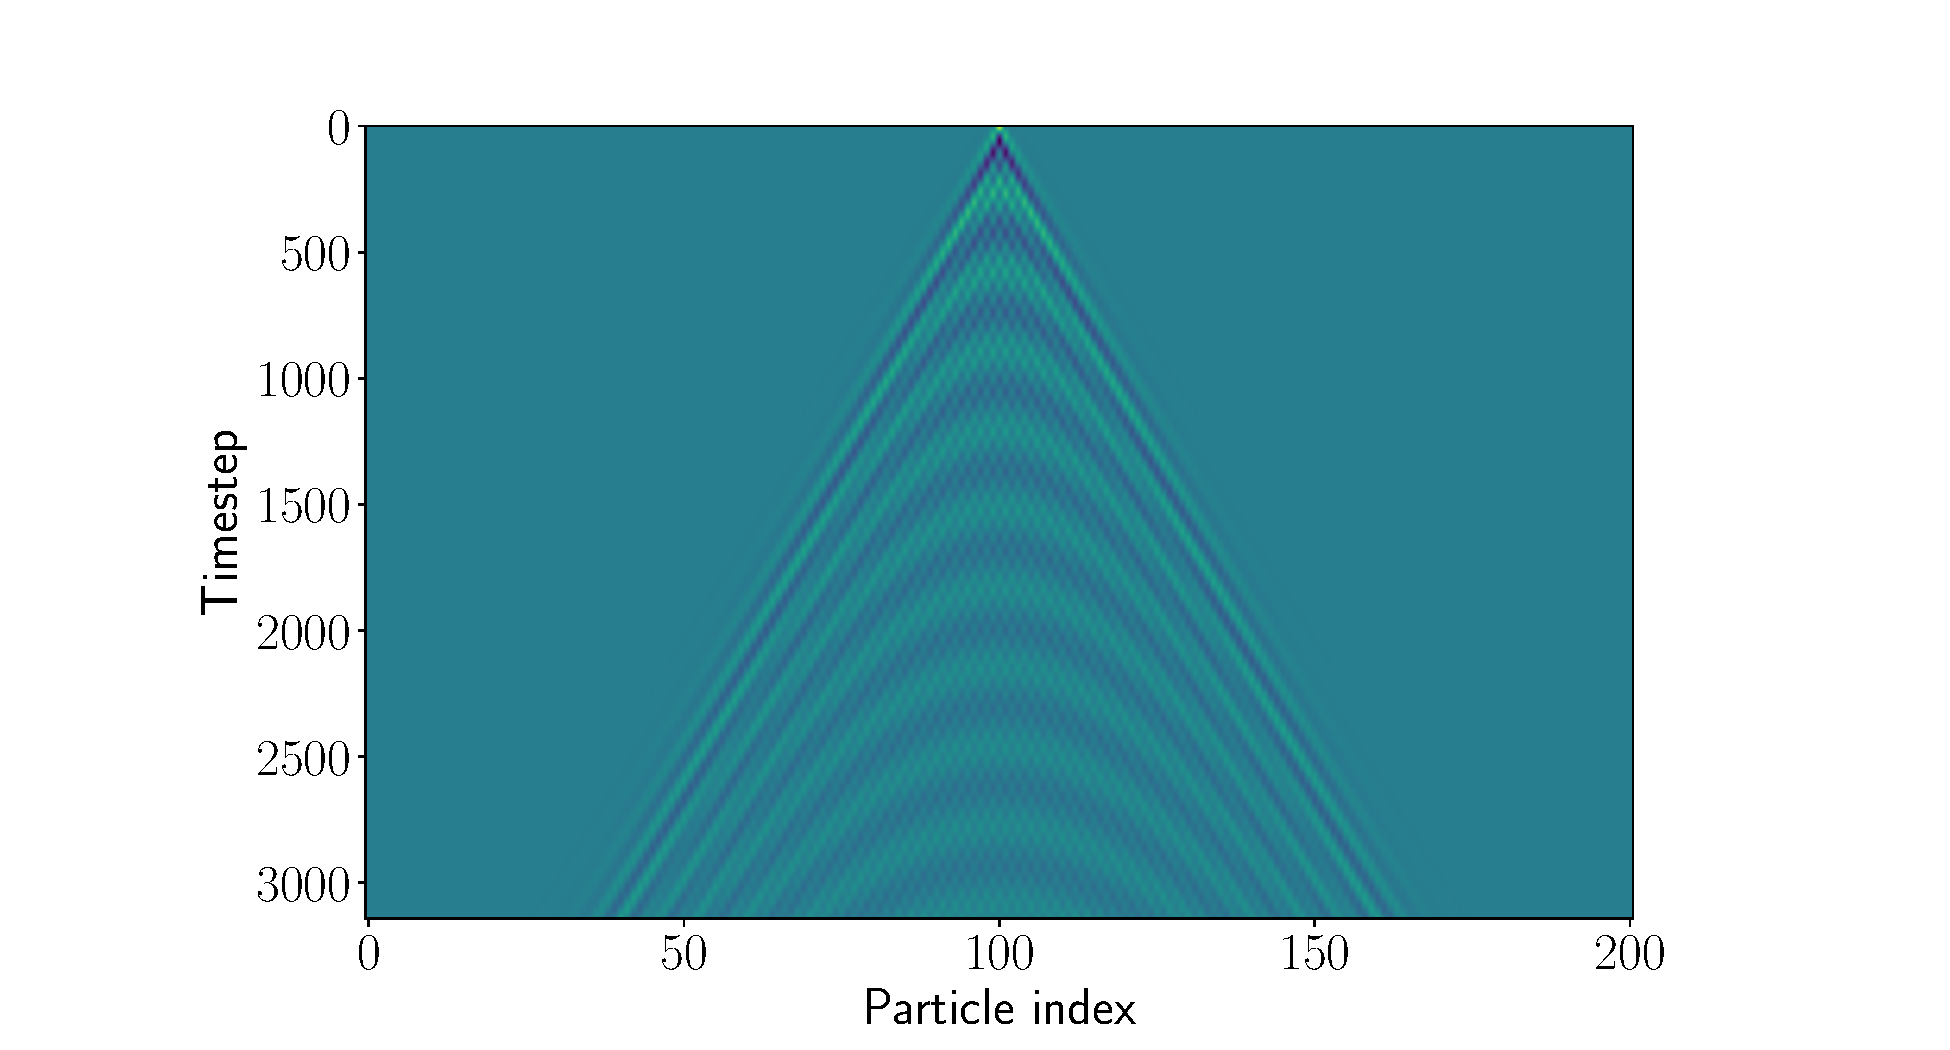
\includegraphics[width=\columnwidth]{../fig/wave_200.pdf}
	\caption{The figure shows the amplitudes of coupled oscillations of $201$ spins.}
	\label{fig:200_heat}
\end{figure}

\subsubsection{Damped, coupled system}

Based on the results from including damping on one spin and the behaviour of the magnon in the previous section we would expect the damped coupled system to show a collective wave motion whose amplitude eventually dies out. This is exactly what is observed in \href{https://folk.ntnu.no/sondrdl/spinwaves/coupled_spins_damped.mp4}{this} video showing the time evolution of the system when we set $\alpha = 0.1$. A heat map illustrating the same time evolution only with slightly less damping is shown in figure \ref{fig:damped_heat}. Here it is evident that the oscillations die out in the case of $\alpha = 0.05$ while they continue to propagate when $\alpha = 0$. Notice also that due to the periodic boundary conditions, there are two magnons propagating through the system. This is observed in the plot as the zigzag pattern, while in the video it is clear from the start that the initial perturbation also affects the last spin in the chain.

\begin{figure}[htb]
	\centering
	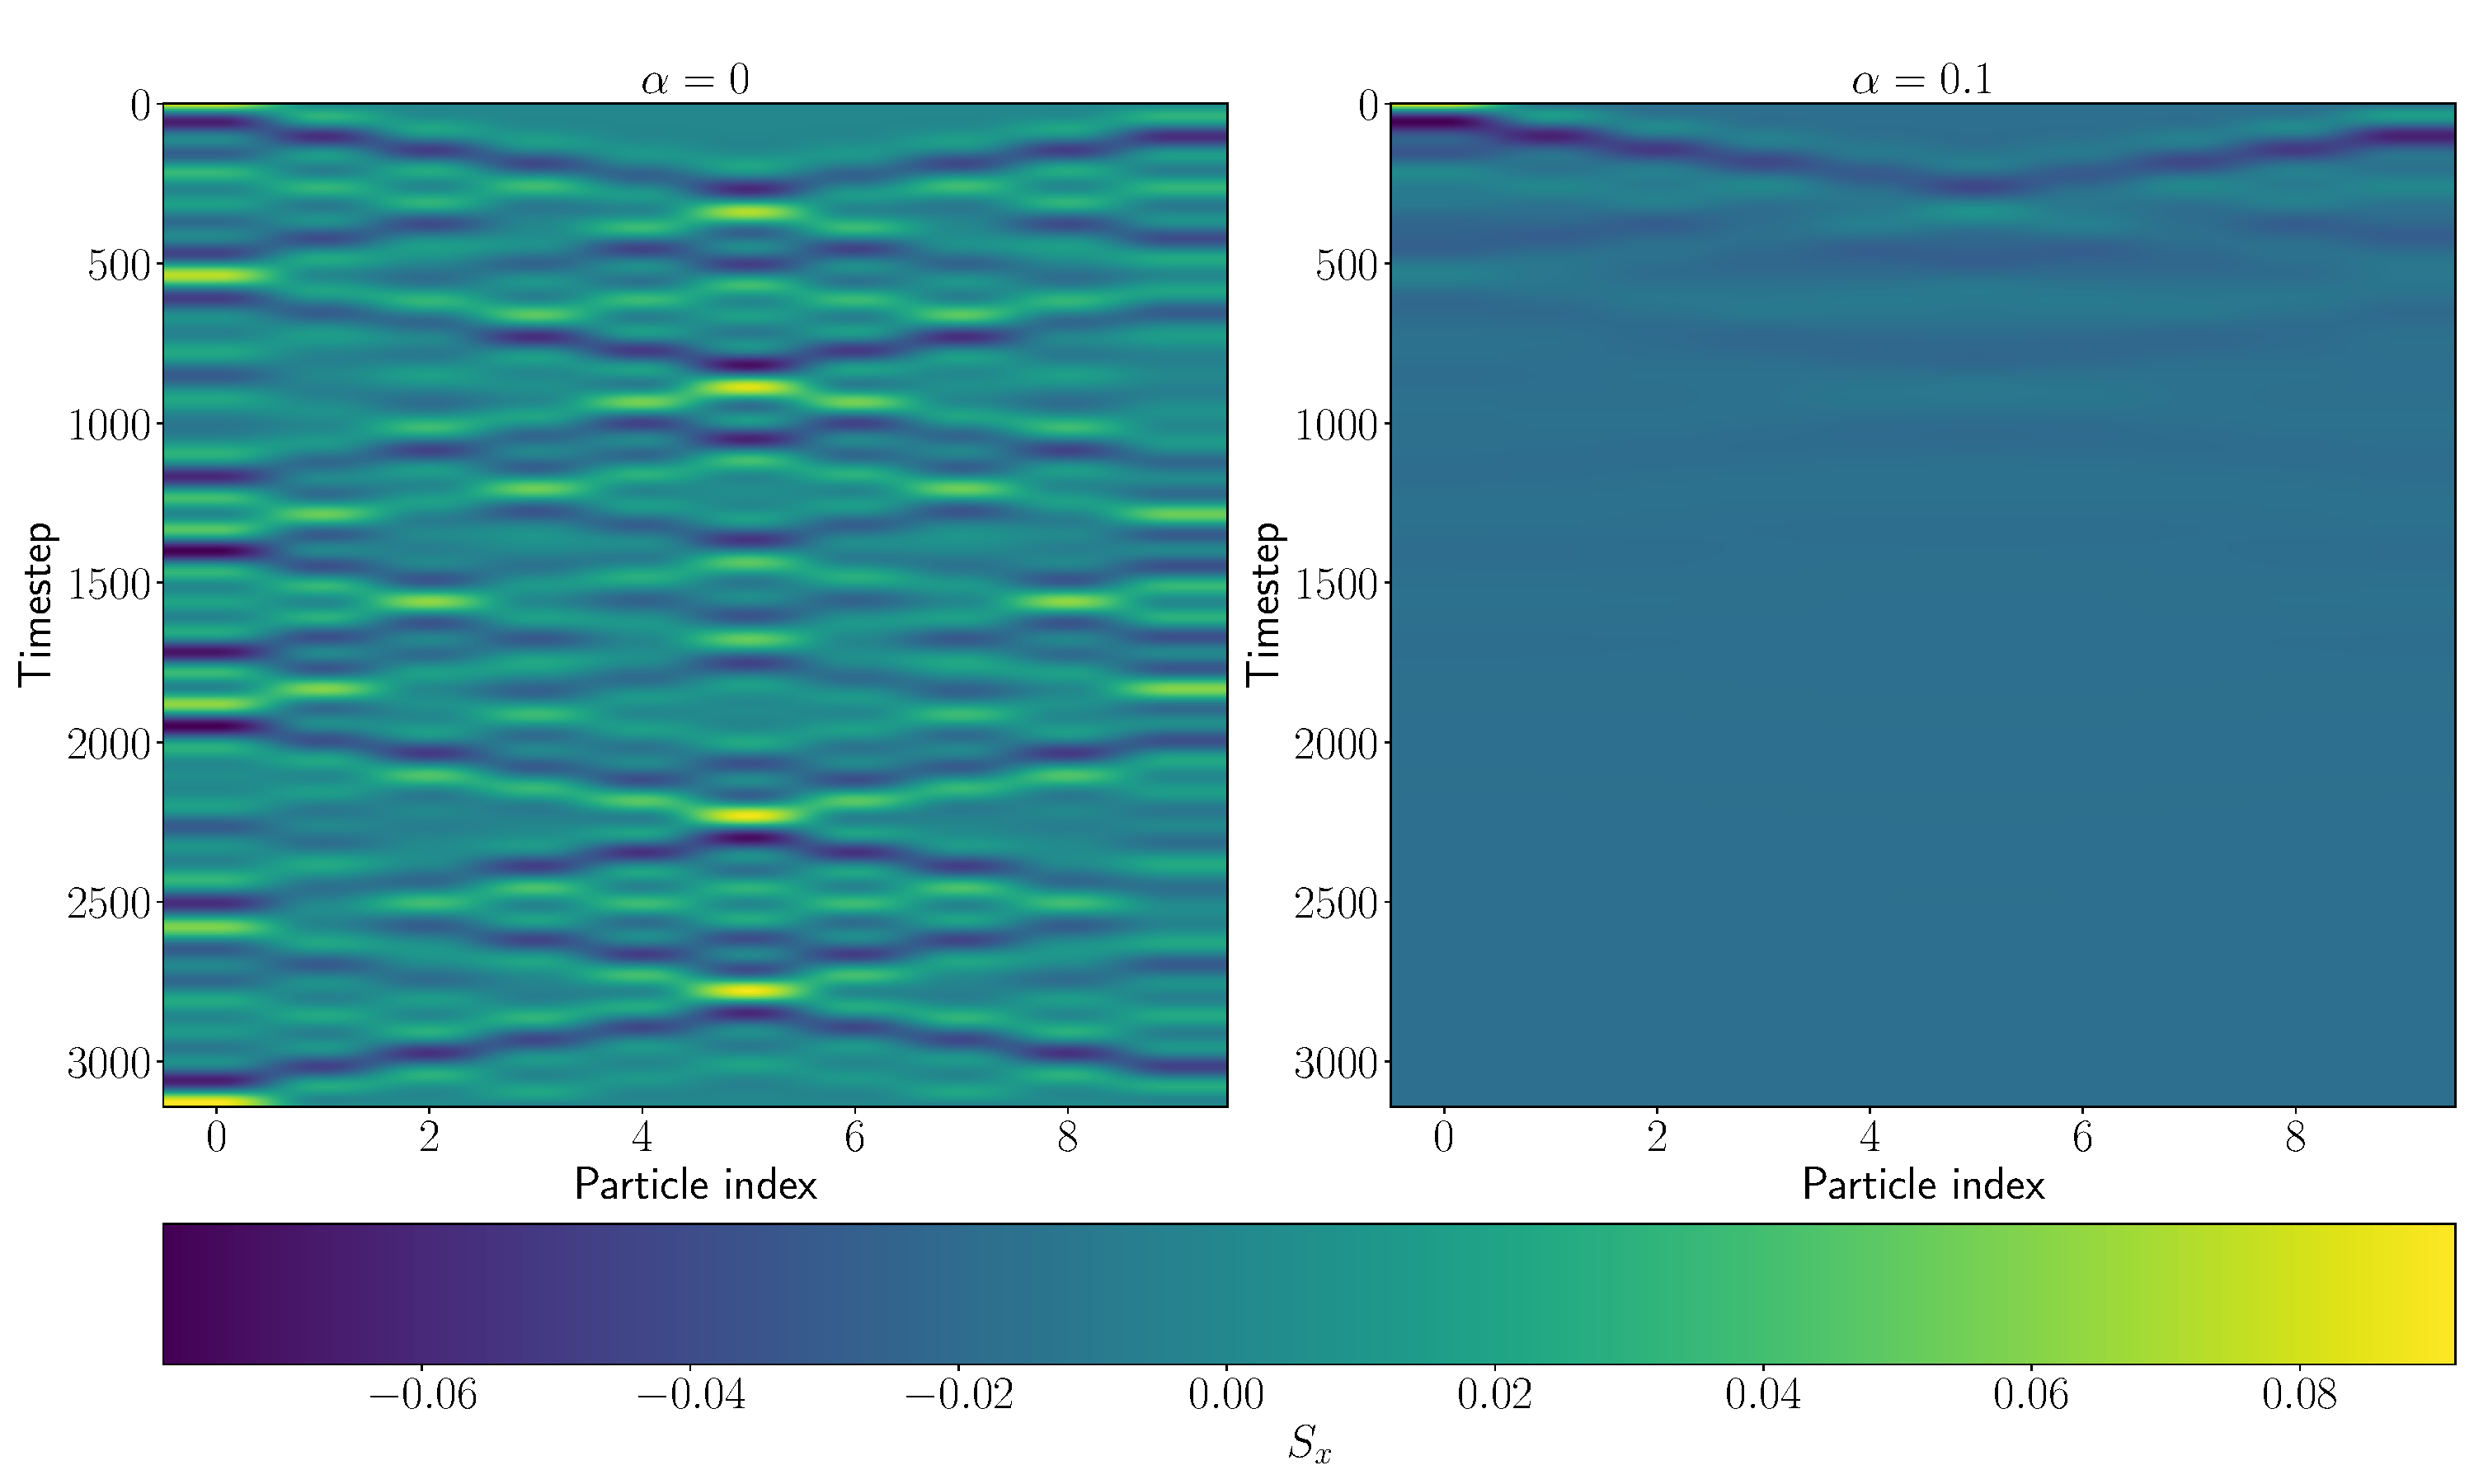
\includegraphics[width=\columnwidth]{../fig/damped_vs_undamped.pdf}
	\caption{The figure shows the amplitudes of coupled oscillations of the spins for $\alpha = 0$ and $\alpha = 0.05$ given the same initial conditions.}
	\label{fig:damped_heat}
\end{figure}

\subsubsection{Antiferromagnetic coupling, $J<0$}

The case of $J<0$ is very similar to the case considered in \ref{sec:groundstates}. The video of the time evolution corresponding to this case can be found \href{https://folk.ntnu.no/sondrdl/spinwaves/coupled_spins_anti.mp4}{here}. As one spin is tilted, the neighbours tend to oscillate in phase with their neighbours as opposed to the ferromagnetic case where the spins are repelled by their neighbours. 

\subsubsection{Magnetisation}

In section \ref{sec:groundstates} there is a net magnetisation only in the case where $J>0$, whereas it is zero when $J<0$. In the first case the magnetisation is either $-1$ or $1$, depending on the sign of the anisotropy constant $d_z$. In our case $d_z < 0$ so the equilibrium magnetisation is $-1$\footnote{This rather flimsily defined magnetisation we refer to is meant to be the average of the $z$-components of each spin.}. For the case of $J<0$, half of the spins will align along $+\mathbf{e}_z$ and the other half along $-\mathbf{e}_z$ as explained in section \ref{sec:groundstates}.